% !TeX spellcheck = en_GB
\documentclass[usenames,dvipsnames,aspectratio=169]{beamer}
\usepackage{tcolorbox} % Add this package
\usepackage{tikz}
\usetikzlibrary{shadows} % Load the shadows library
\usepackage{graphicx}
\usetheme{Szeged}
\usecolortheme{beaver}


% Define custom colors for Elixir
\definecolor{ElixirPurple}{RGB}{104, 55, 155} % Adjust the RGB values to match Elixir's purple
\definecolor{ElixirLightPurple}{RGB}{170, 120, 210} % A lighter shade of purple
\definecolor{ElixirVeryLightPurple}{RGB}{230, 220, 250} % A very light shade of purple for the background


% Setting color of bars
% Setting colors for the bars and title
\setbeamercolor{palette primary}{bg=ElixirPurple,fg=white}
\setbeamercolor{palette secondary}{bg=ElixirLightPurple,fg=white}
\setbeamercolor{palette tertiary}{bg=ElixirPurple,fg=white}
\setbeamercolor{palette quaternary}{bg=ElixirPurple,fg=white}
\setbeamercolor{titlelike}{parent=palette primary, fg=white}
\setbeamercolor{frametitle}{fg=white,bg=ElixirPurple}
\setbeamercolor{background canvas}{bg=ElixirVeryLightPurple}


% Set item colors
\setbeamercolor{item}{fg=ElixirPurple}
\setbeamercolor{itemize item}{fg=ElixirPurple}
\setbeamercolor{itemize subitem}{fg=ElixirPurple}


\title{Sentiment Analysis on Mastodon Posts}
\subtitle{Predicting Election Outcomes with Elixir?}
\author{Sebastian Heiden}
\institute{Harz University of Applied Sciences}
\date{\today}

\newcommand{\graybar}[4]{
	\begin{tikzpicture}[remember picture, overlay]
		\node at (current page.north west) [anchor=north west, xshift=#1, yshift=#2] {
			\begin{tikzpicture}
				\draw[fill=gray!10, draw=none] (0, 0) rectangle (#3, -#4);
			\end{tikzpicture}
		};
	\end{tikzpicture}
}



% Define a custom command for post-it notes
% Arguments:
% 1: Horizontal shift (positive value moves right, negative left)
% 2: Vertical shift (positive value moves up, negative down)
% 3: Width of the post-it note
% 4: Text to be placed in the post-it note
\newcommand{\postitnote}[4]{
	\begin{tikzpicture}[remember picture, overlay]
		\node[anchor=north west, 
		xshift=#1, 
		yshift=#2, 
		fill=yellow!40, 
		draw=black, 
		thick, 
		text width=#3, 
		rounded corners, 
		drop shadow] 
		at (current page.north west) 
		{#4};
	\end{tikzpicture}
}


\logo{
\includegraphics[height=1cm]{pictures/LogoElixirBerlin.png}} % Adjust size as needed

\begin{document}
	
	{
		\setbeamertemplate{headline}{} % Removes header from title page
		\begin{frame}
			\titlepage
		\end{frame}
	}
	
	% Your other slides go here
	
	\section{About Me}
	\begin{frame}{About Me}
		\begin{columns}
			
			\begin{column}{0.45\textwidth}
				\begin{tcolorbox}[colback=white, colframe=ElixirPurple, arc=3mm, boxrule=0mm, height=0.8\textheight, valign=center, title=Working Live]
					
					\underline{topics}:
					\begin{itemize}
						\item heat demand and PV cadastres
					\end{itemize}
					\underline{using}:
					\begin{itemize}
						\item geodata (Raster, Vector)
						\item Python: GeoPandas, Numpy
						\item land usage; coverage, property register
					\end{itemize}
		
				\end{tcolorbox}
			\end{column}
			
			\begin{column}{0.45\textwidth}
				\begin{tcolorbox}[colback=white, colframe=ElixirPurple, arc=3mm, boxrule=0mm, height=0.8\textheight, valign=center, title=Privat Live]
					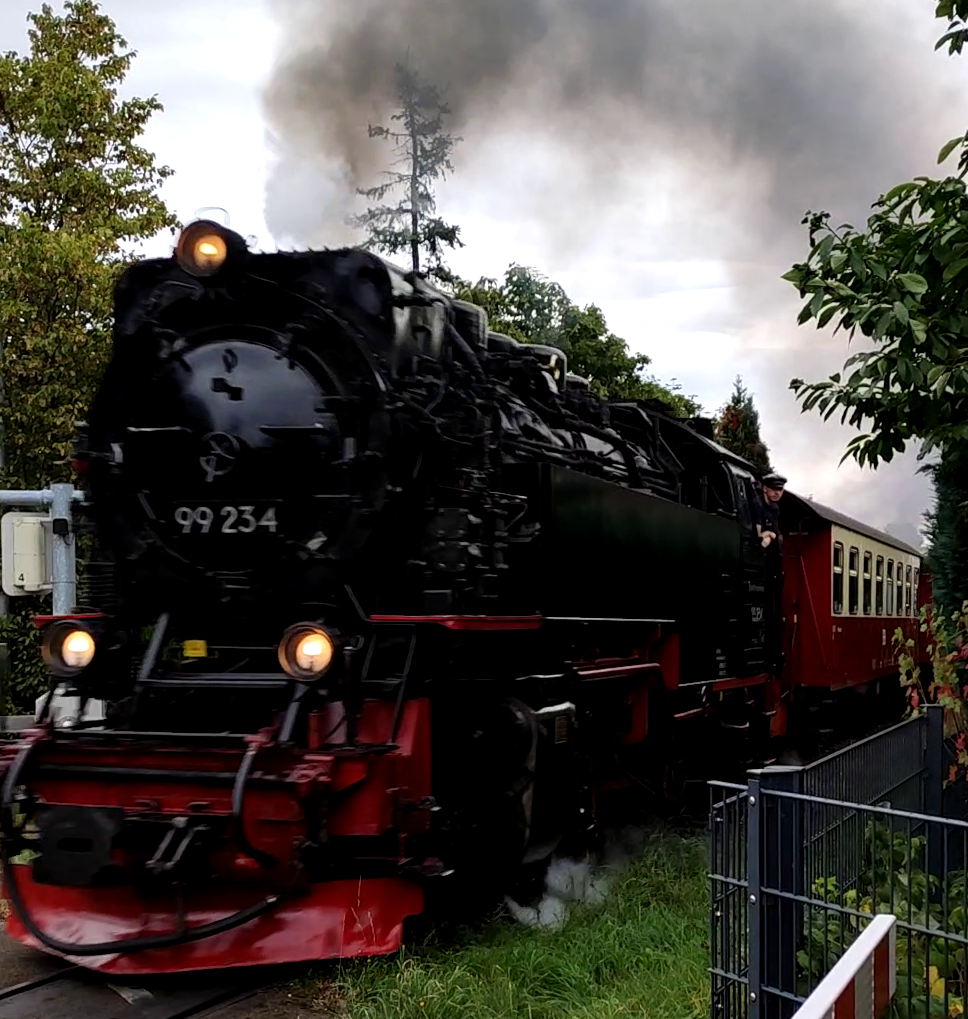
\includegraphics[width=\tcbtextwidth,   keepaspectratio]{pictures/vlcsnap-2024-01-31-23h37m06s479.png}
				\end{tcolorbox}
			\end{column}
			
		\end{columns}
	\end{frame}
	
	\section{Motivation}
	\begin{frame}{Election on Twitter}
		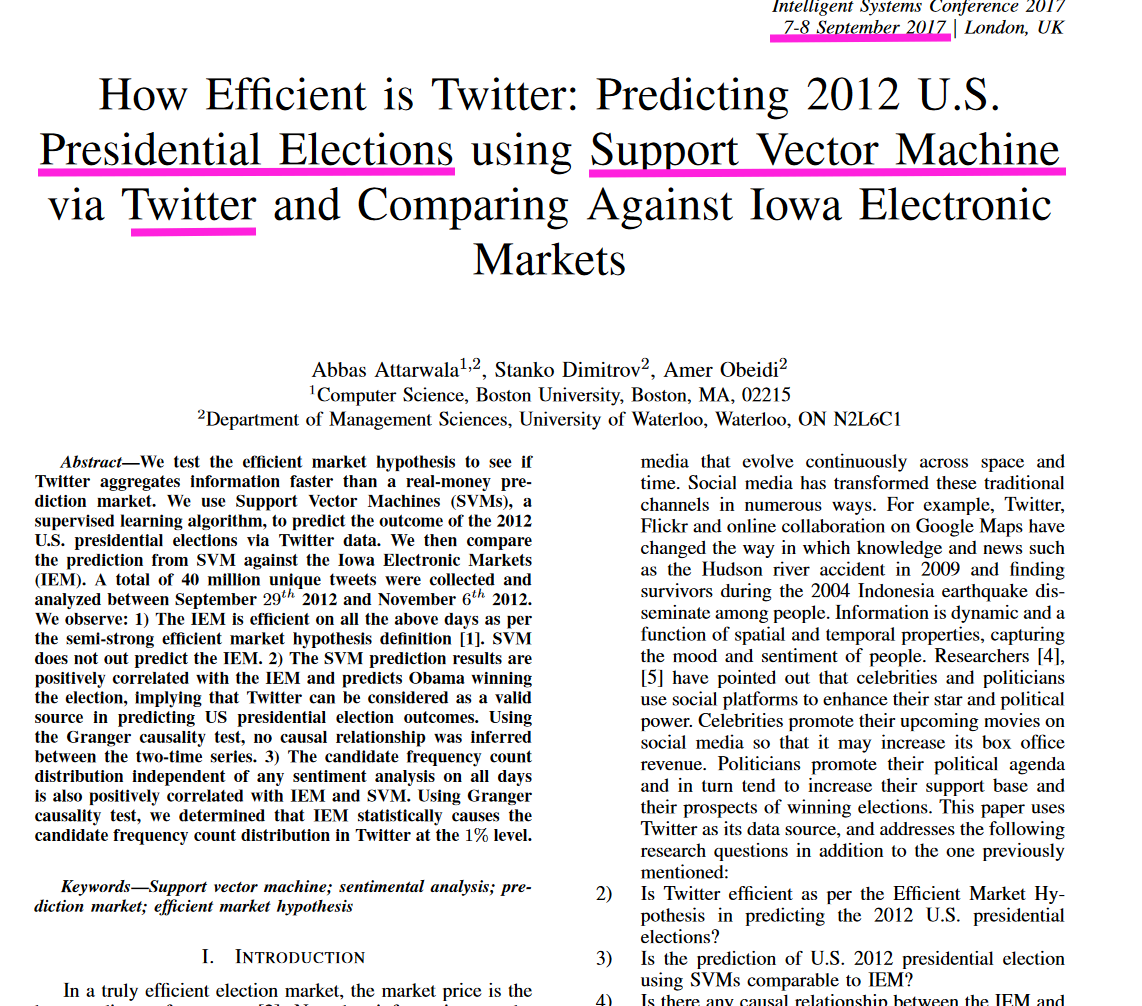
\includegraphics[width=\linewidth, keepaspectratio]{pictures/TwitterElection2012/Twitter_Election_2012.png}
	\end{frame}
	

	\begin{frame}{Prediction}
	\begin{columns}
	
	\begin{column}{0.45\textwidth}
		\begin{tcolorbox}[colback=white, colframe=ElixirPurple, arc=3mm, boxrule=0mm, height=0.8\textheight, valign=center, title=Frequency]
				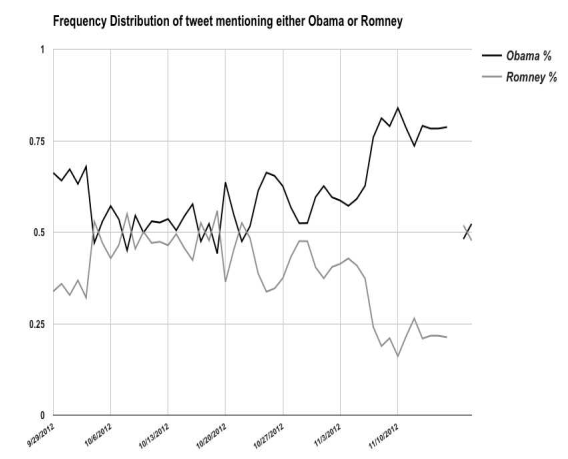
\includegraphics[width=\tcbtextwidth,   keepaspectratio]{pictures/TwitterElection2012/twitter_temp_distr.png}
		\end{tcolorbox}
	\end{column}
	
	\begin{column}{0.45\textwidth}
		\begin{tcolorbox}[colback=white, colframe=ElixirPurple, arc=3mm, boxrule=0mm, height=0.8\textheight, valign=center, title=Prediction]
			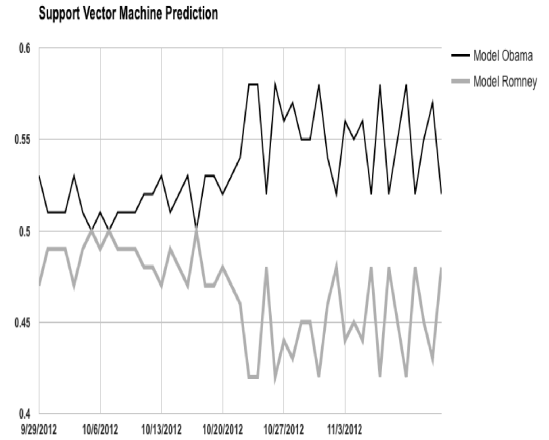
\includegraphics[width=\tcbtextwidth,   keepaspectratio]{pictures/TwitterElection2012/twitter_svm.png}
		\end{tcolorbox}
	\end{column}
	
	\end{columns}
	\end{frame}
	
	
	\begin{frame}{Election on Mastodon}
		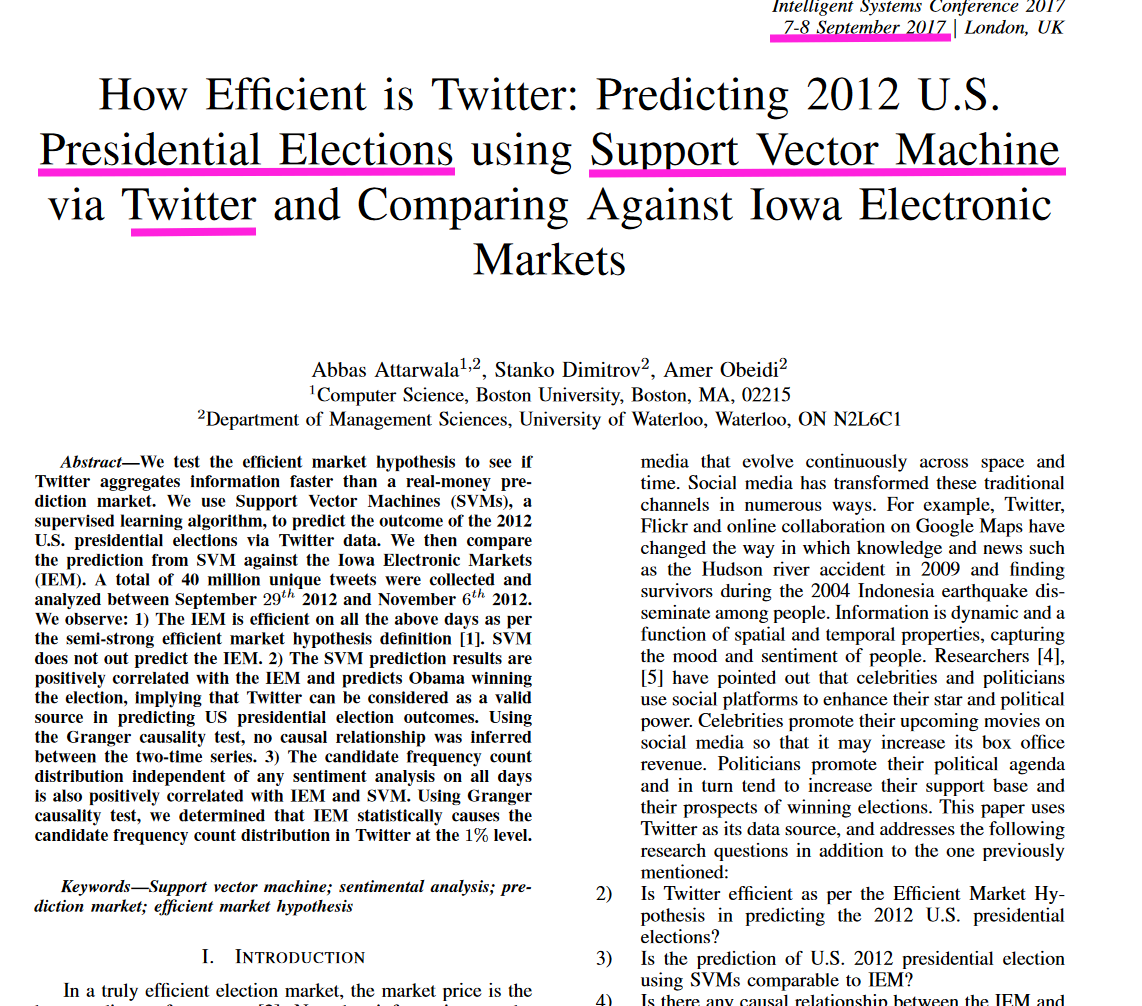
\includegraphics[width=\linewidth, keepaspectratio]{pictures/TwitterElection2012/Twitter_Election_2012.png}
		\postitnote{1.5cm}{-3.5cm}{4.8cm}{Bavarian State Election}
		\postitnote{8.2cm}{-3.5cm}{6.5cm}{Pre-Trained Deep Learning NLP Model}
		
		
		\postitnote{6.1cm}{-2.8cm}{1.8cm}{Mastodon}
		\postitnote{10.8cm}{-2.8cm}{2.5cm}{2023}
		
		 \graybar{4.1cm}{-4.1cm}{10.8cm}{2.0cm}
		 \postitnote{2.3cm}{-4.2cm}{1.8cm}{Mastodon}

	\end{frame}
	
	\section{DS Background}
	
	\begin{frame}{Data Science \& Big Data}
		\begin{columns}
			
			\begin{column}{0.45\textwidth}
				\begin{tcolorbox}[colback=white, colframe=ElixirPurple, arc=3mm, boxrule=0mm, height=0.8\textheight, valign=center, title=DS Perspective]
					\includegraphics[width=\tcbtextwidth,   keepaspectratio]{pictures/high_level.png}
				\end{tcolorbox}
			\end{column}
			
			\begin{column}{0.45\textwidth}
				\begin{tcolorbox}[colback=white, colframe=ElixirPurple, arc=3mm, boxrule=0mm, height=0.8\textheight, valign=center, title=Big Data]
					
					\begin{itemize}
						\item Volumne
						\item Velocity
						\item Variety
						\hrule
						\item Varacity
						\hrule
						\item Value
						\item Validity
					
					\end{itemize}
					
				\end{tcolorbox}
			\end{column}
		\end{columns}
	\end{frame}
	
	\begin{frame}{CRISP-DM}
		\includegraphics[width=\linewidth, keepaspectratio]{pictures/crisp_dm.png}
	\end{frame}
	
	\section{Lets Get some Data}
	\begin{frame}{Research Question}
		
		Predict the voting result of the 2023 Bavarian State election with Mastadon.
		
		\begin{itemize}
			\item time period: six weeks
			\item  
		\end{itemize}
		
	\end{frame}
	
	\begin{frame}{Sourcing}
		
		\begin{itemize}
			\item Search: {{instance\_url}}\/api\/v1\/timelines\/tag/{{tag\_name}}
			\begin{itemize}
				\item opt-in
				\item finished role out 2 days before election
			\end{itemize}
			\item Tags: {{isntance\_url}}\/api\/v2\/search?q={{search\_word}}
			\begin{itemize}
				\item used public timeline
			\end{itemize}
			
		\end{itemize}
	\end{frame}
	
	\begin{frame}{Data Understanding}
	\end{frame}
	
	\begin{frame}{Data Cleaning}
		\begin{columns}
			
			\begin{column}{0.45\textwidth}
				\begin{tcolorbox}[colback=white, colframe=ElixirPurple, arc=3mm, boxrule=0mm, height=0.8\textheight, valign=center, title=Text Cleaning]
				\end{tcolorbox}
			\end{column}
			
			\begin{column}{0.45\textwidth}
				\begin{tcolorbox}[colback=white, colframe=ElixirPurple, arc=3mm, boxrule=0mm, height=0.8\textheight, valign=center, title=Post Selection]
					
					
				\end{tcolorbox}
			\end{column}
		\end{columns}
	\end{frame}
	
	\section{Lets Get some Data}
	\begin{frame}{Polls CSU}
		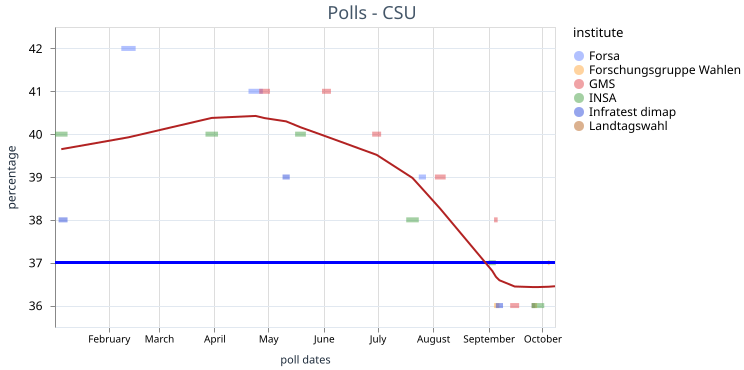
\includegraphics[width=\linewidth, keepaspectratio]{pictures/paper/polls/visualization_csu_polls.png}
	\end{frame}
	
	\begin{frame}{Polls CSU}
		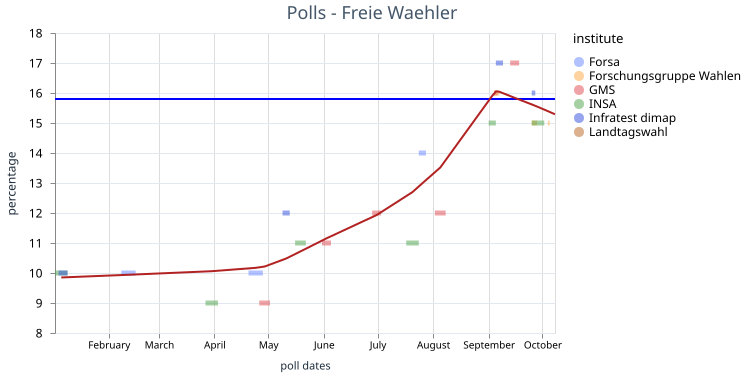
\includegraphics[width=\linewidth, keepaspectratio]{pictures/paper/polls/visualization_fw_polls.png}
	\end{frame}
	
	\begin{frame}{Post Frequencies}
		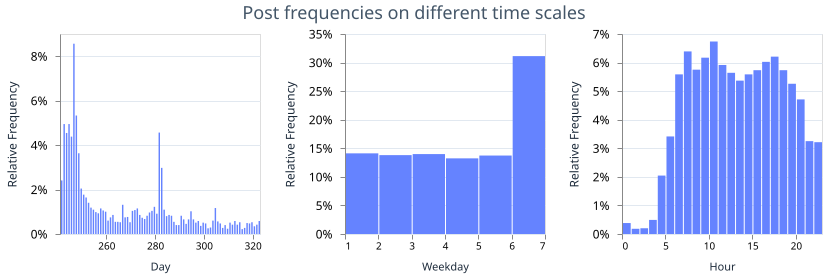
\includegraphics[width=\linewidth, keepaspectratio]{pictures/paper/sentiments/visualization_valid_posts_frequency.png}
	\end{frame}
	
	
\end{document}

